% Frozen v3 Physics-versus-Zbb BDT review, 2026-10-03.
\documentclass[aspectratio=169,10pt]{beamer}
\usetheme{Boadilla}
\usepackage{booktabs}
\usepackage{graphicx}
\usepackage{amsmath}
\definecolor{navy}{HTML}{17365D}
\setbeamercolor{structure}{fg=navy}
\setbeamercolor{frametitle}{fg=navy}
\setbeamertemplate{navigation symbols}{}
\setbeamertemplate{footline}[frame number]
\graphicspath{{figures/}}
\newcommand{\Lb}{\Lambda_b}
\newcommand{\Lz}{\Lambda^0}
\newcommand{\smallsource}[1]{\vfill{\tiny\color{gray}#1}}

\title{\texorpdfstring{$\Lb\to\Lz\gamma$}{Lb to Lambda gamma}: v3 BDT review}
\subtitle{Frozen 1,028-chunk Physics versus inclusive $Z\to b\bar b$ snapshot}
\author{Renato Quagliani}
\institute{FCC-ee analysis review}
\date{3 October 2026}

\begin{document}
\begin{frame}
\titlepage
\begin{center}\small Validation scan and independent-test projection; score is a proposal for PI review.\end{center}
\end{frame}

\begin{frame}{Frozen inputs and candidate cutflow}
\begin{columns}[T]
\begin{column}{.54\textwidth}
\small
\begin{tabular}{lrr}
\toprule
Candidate stage & Direct signal & Zbb other\\
\midrule
Stage 1 & 55,395 & 5,935,608\\
Fit check & 55,395 & 4,843,426\\
$\Lz$ check & 55,264 & 4,401,877\\
Offline selected & 54,872 & 1,060,544\\
\bottomrule
\end{tabular}
\vspace{.4cm}

\begin{itemize}
\item 100,000 signal input events; generator audit counts 100,002 direct decays.
\item 376,723,929 processed Zbb events in 1,028 valid v3 chunks; 172 of 1,200 jobs missing at freeze.
\item Offline: $|m(p\pi)-m_{\Lz}|\leq12.5$ MeV, $E(\Lb)\geq10.5$ GeV, same thrust hemisphere; no photon veto.
\end{itemize}
\end{column}
\begin{column}{.44\textwidth}
\begin{block}{Normalization}
\small $S=816642\,(N_{\rm direct}/N_{\rm gen\ events})$\\[.15cm]
$B=9\times10^{11}\,(N_{\rm Zbb\ other}/N_{\rm processed\ Zbb})$
\end{block}
\small Candidate yields in the full $4.7$--$6.5$ GeV mass interval. One forced decay/event is the code approximation; two input events contain an extra direct chain.
\end{column}
\end{columns}
\smallsource{Full cutflow with conditional and cumulative retention: docs/STAGE2\_V3\_BDT\_REVIEW\_2026-10-03.md; frozen catalog and preparation summary in docs/data/stage2\_v3\_bdt\_1028.}
\end{frame}

\begin{frame}{One reconstructed event: topology and isolation}
\centering
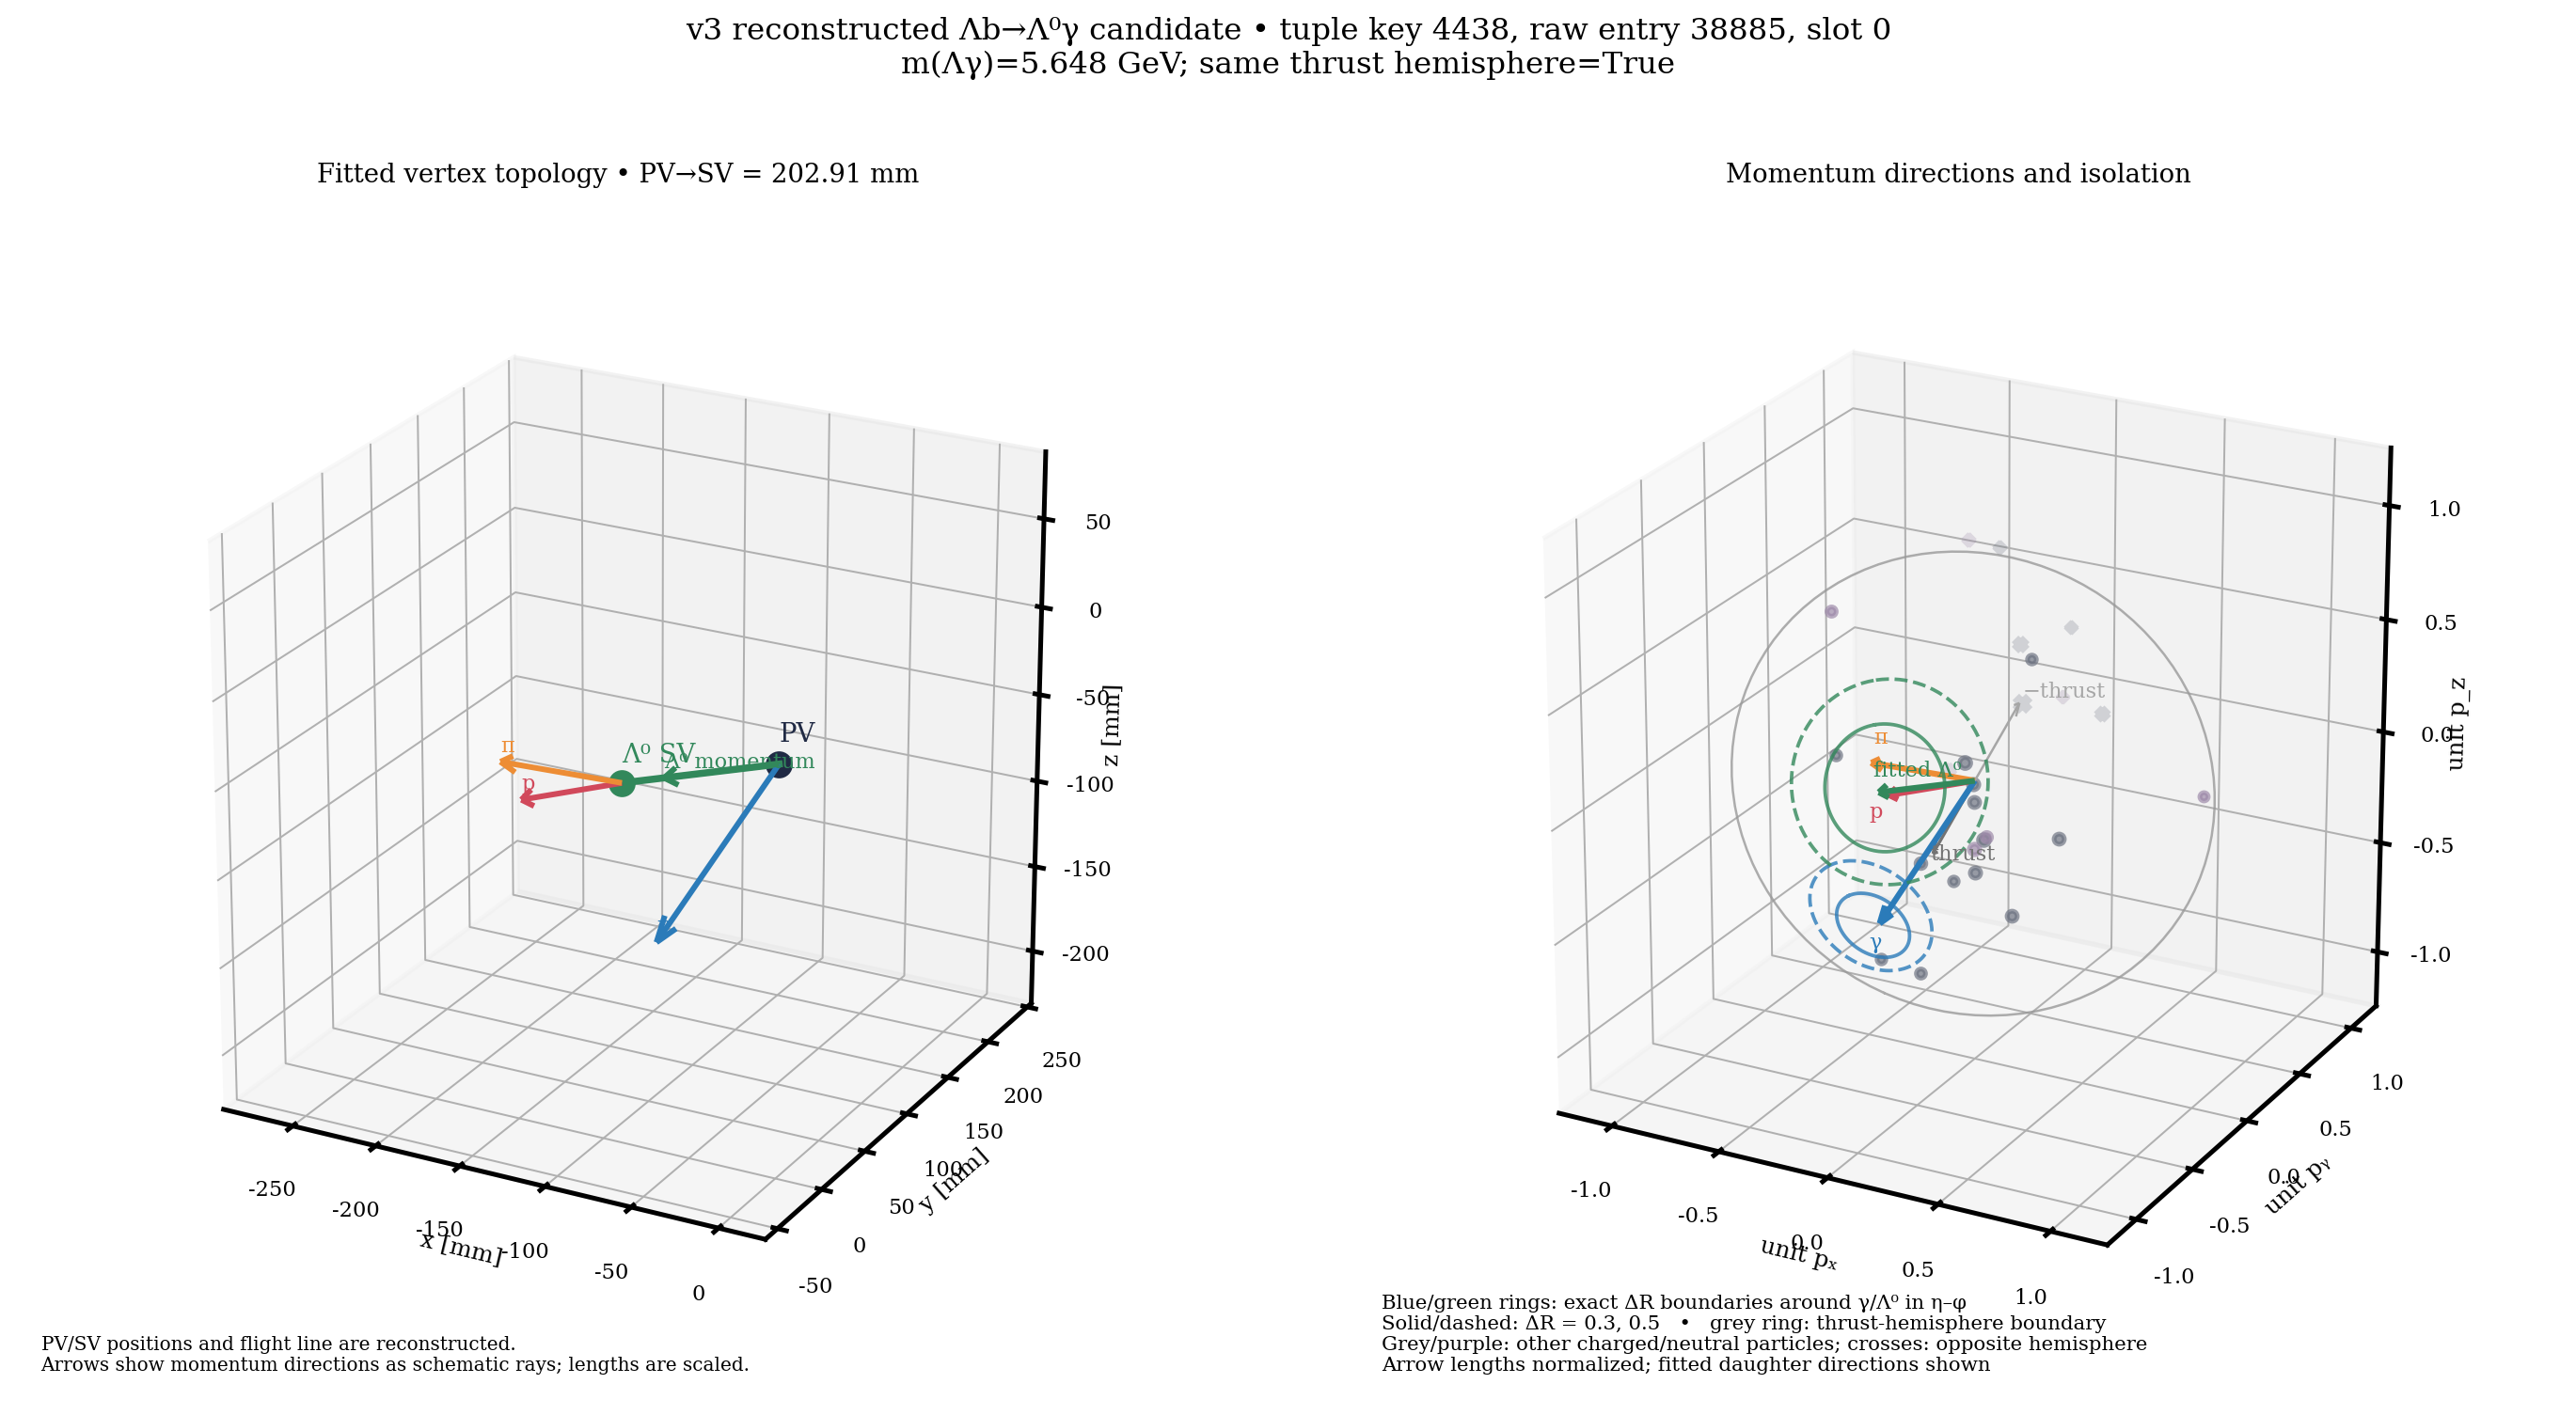
\includegraphics[width=.99\textwidth,height=.82\textheight,keepaspectratio]{candidate_3d_view_a.png}
\smallsource{PV and fitted $\Lz$ SV in mm; $\Delta R$ boundaries are mapped from $\eta$--$\phi$ into direction space. One event for explanation, not an efficiency measurement.}
\end{frame}

\begin{frame}{Held-out response}
\begin{columns}[T]
\begin{column}{.52\textwidth}
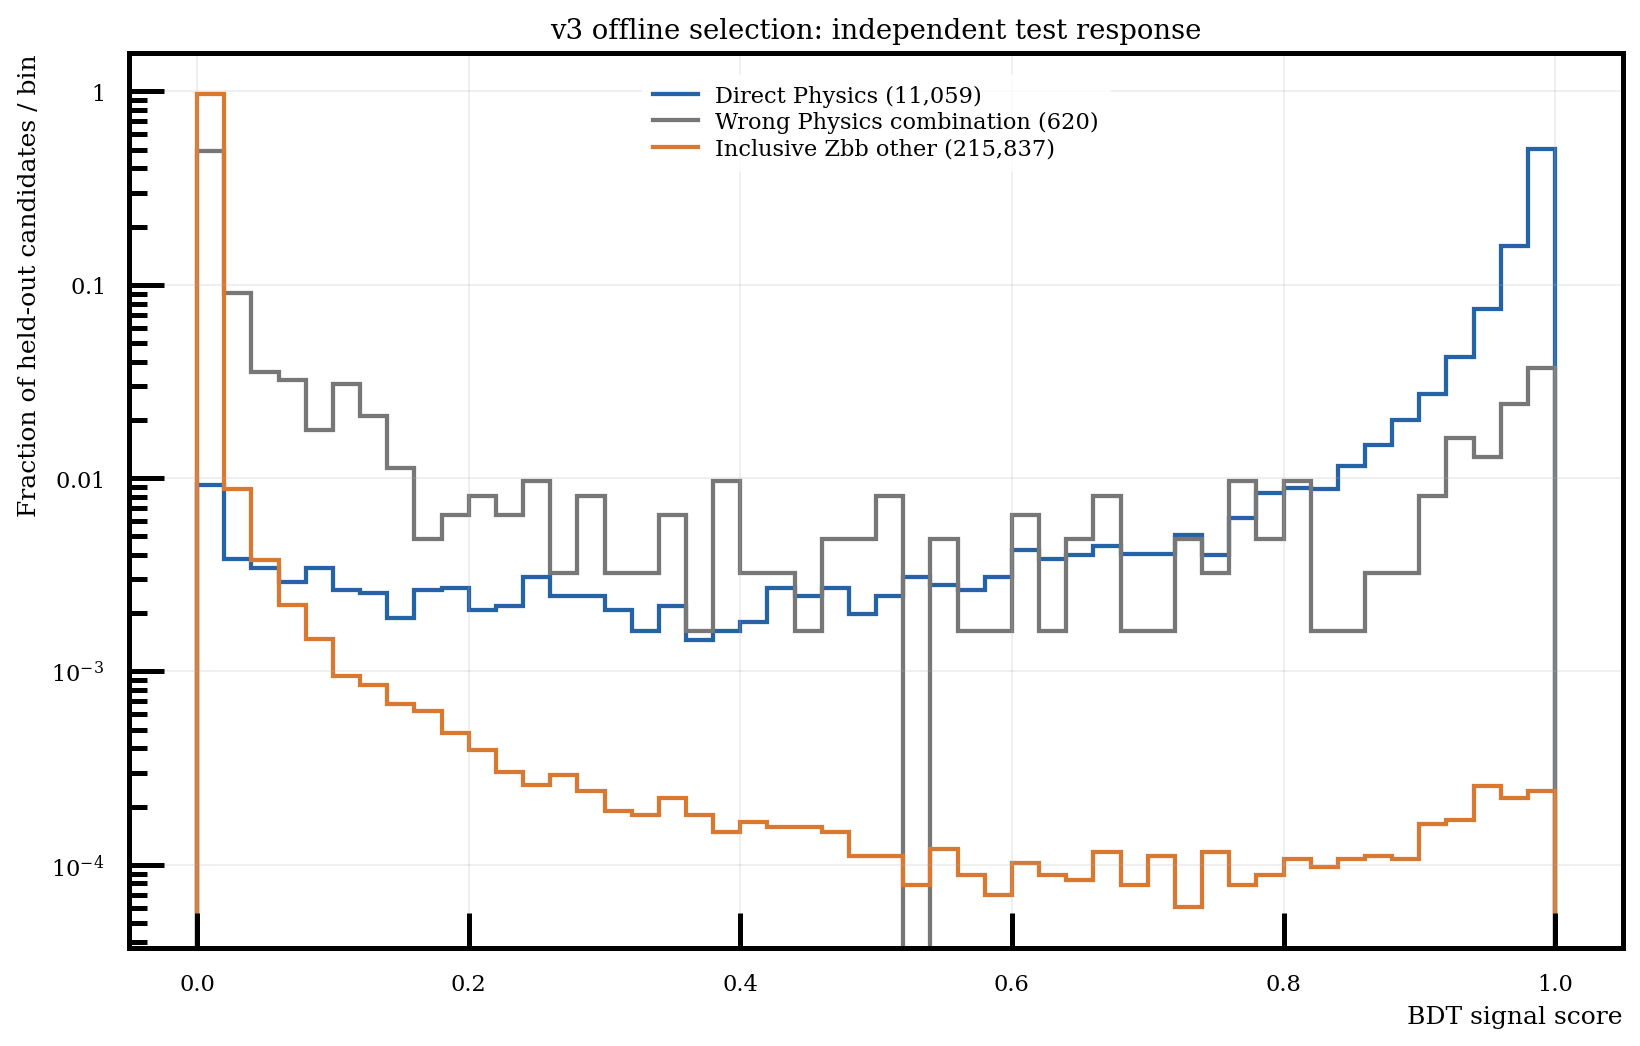
\includegraphics[width=\textwidth]{test_response_three_categories.png}
\end{column}
\begin{column}{.46\textwidth}
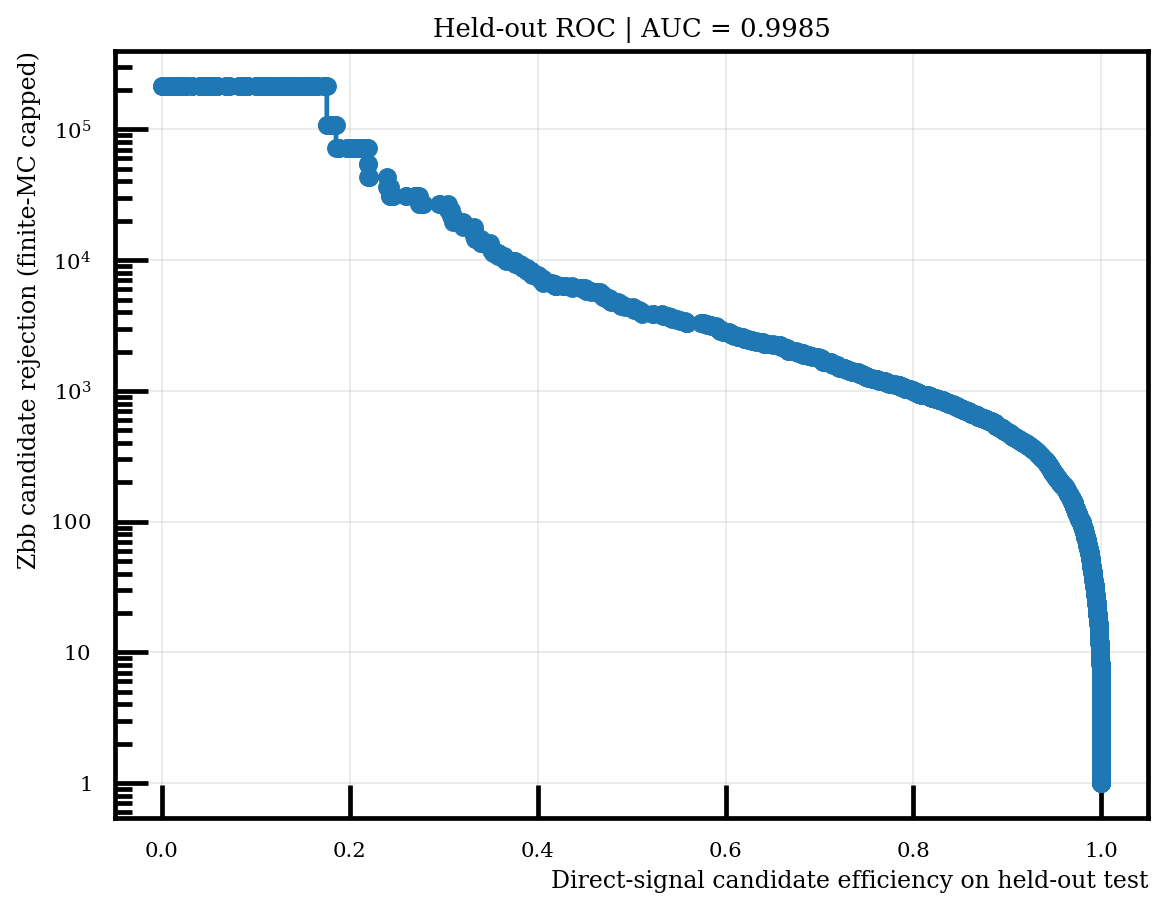
\includegraphics[width=\textwidth]{test_roc.png}
\end{column}
\end{columns}
\small 20 named reconstructed features; no mass, helicity angle, truth, event key, or charge sign in the fit. Train/validation/test AUC: 0.99874 / 0.99864 / 0.99853. The tail rate still depends on observed background counts.
\smallsource{Model: docs/data/stage2\_v3\_bdt\_1028/bdt\_model.json; training summary in the same directory.}
\end{frame}

\begin{frame}{Validation score scan}
\centering
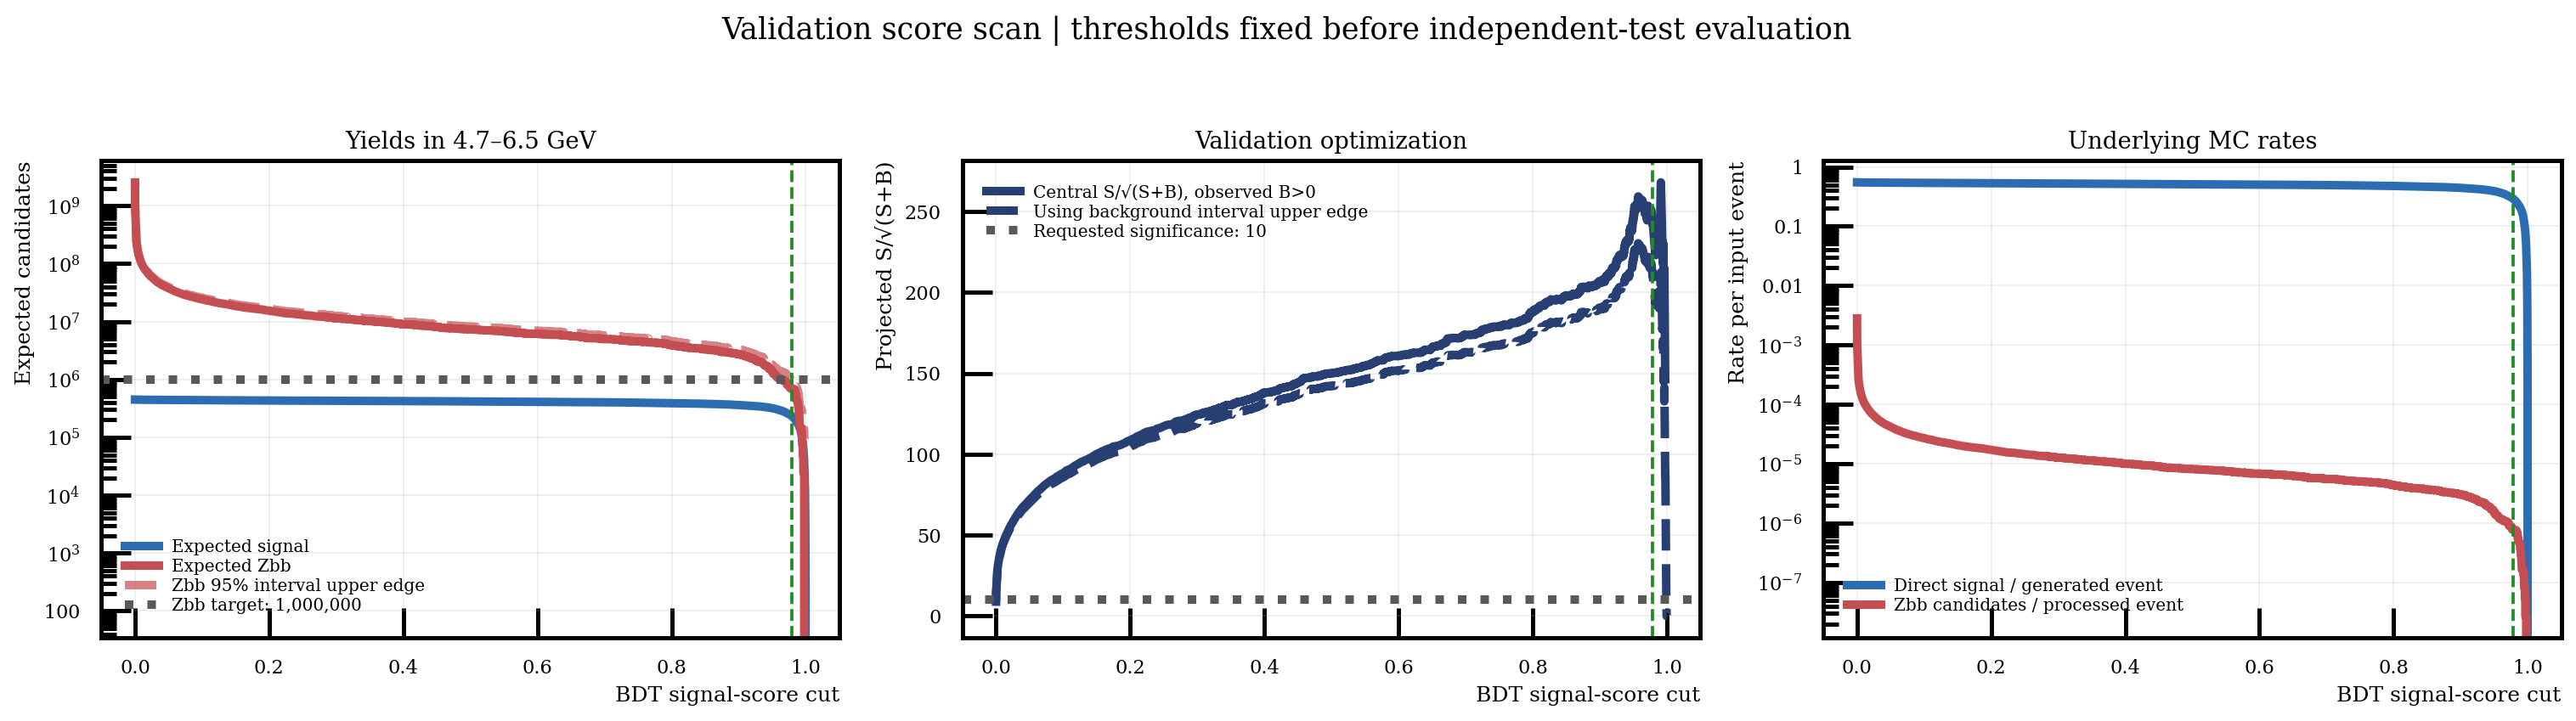
\includegraphics[width=\textwidth,height=.75\textheight,keepaspectratio]{working_point_scan.png}
\smallsource{1,760 validation thresholds include dense near-one scores and exact background order statistics. Green: constrained inspection proposal at score $\geq0.9787055$.}
\end{frame}

\begin{frame}{Tight tail: background count limits}
\centering
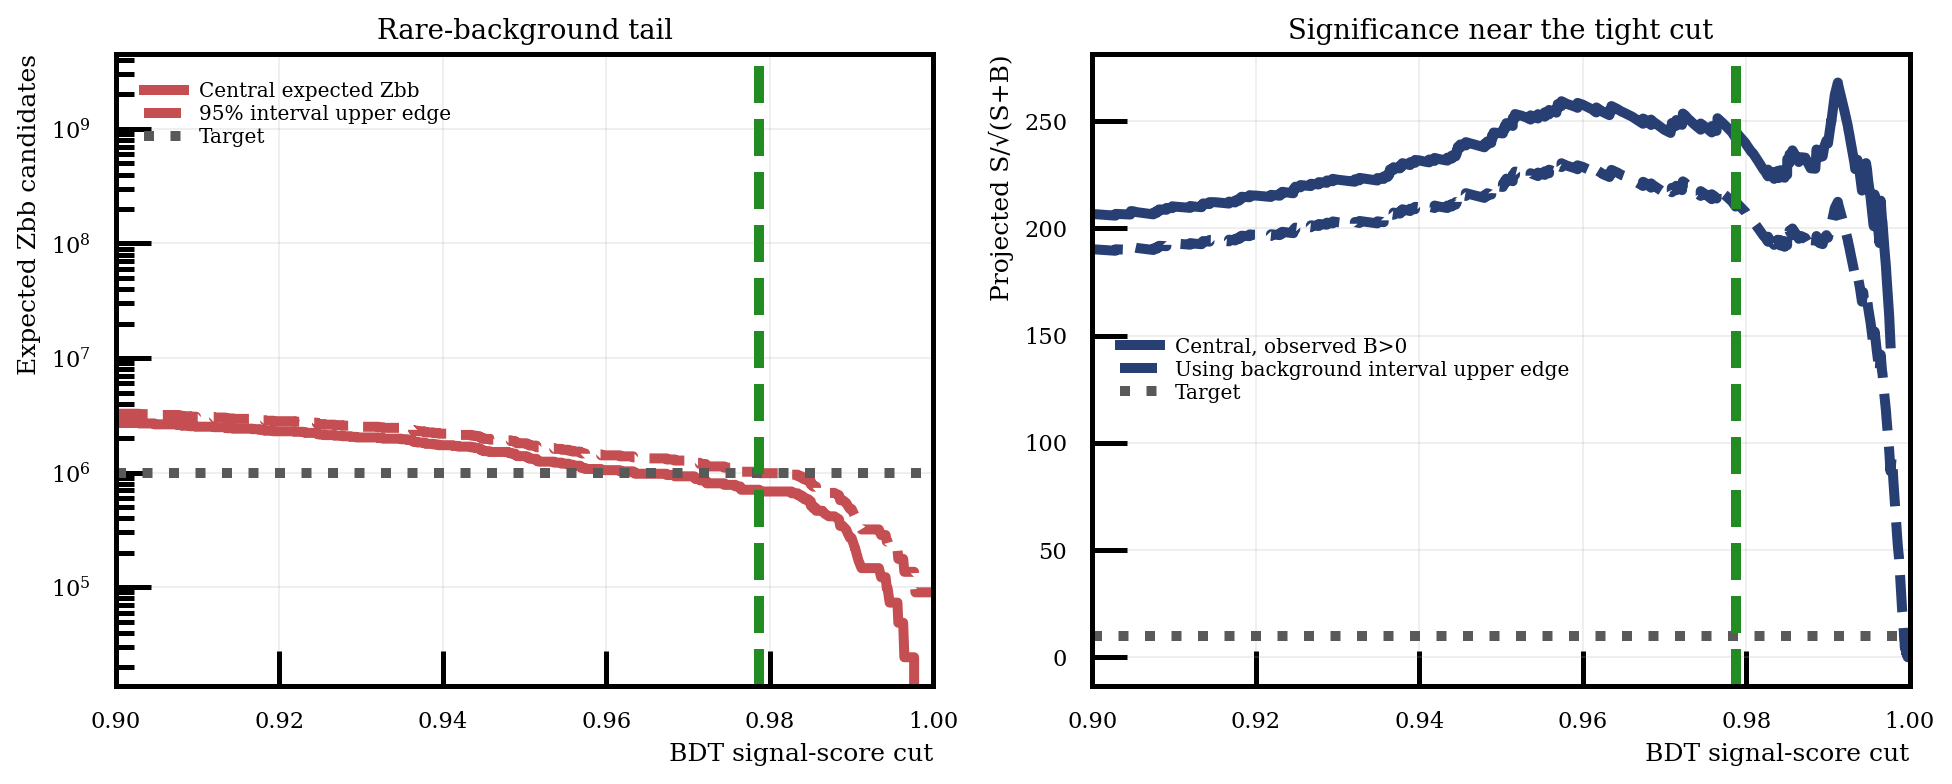
\includegraphics[width=\textwidth,height=.76\textheight,keepaspectratio]{working_point_tail.png}
\smallsource{Validation requires at least 20 observed Zbb candidates and an upper 95\% expected B of at most one million for the marked proposal. A zero-MC tail is unresolved.}
\end{frame}

\begin{frame}{Purity does not yet reach the target}
\centering
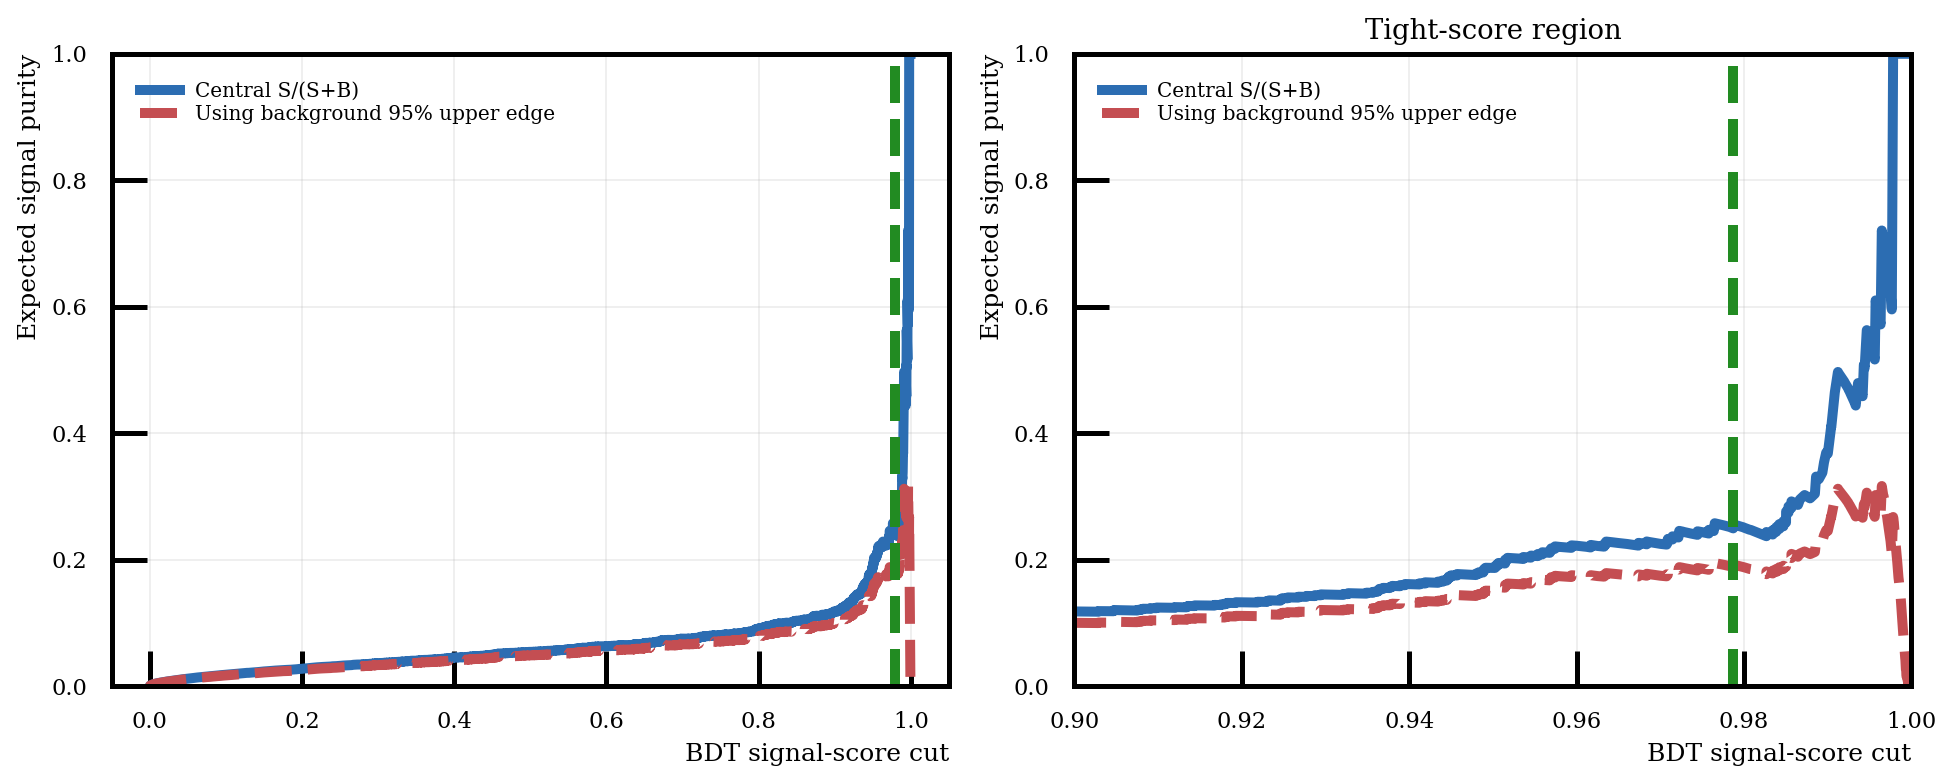
\includegraphics[width=\textwidth,height=.75\textheight,keepaspectratio]{working_point_purity.png}
\smallsource{At score 0.995, only 3 validation Zbb candidates remain: central purity 54.8\%, purity with 95\% upper B 29.3\%. At 0.999, zero observed B does not establish 100\% purity.}
\end{frame}

\begin{frame}{Independent test at the validation-fixed proposal}
\begin{columns}[T]
\begin{column}{.56\textwidth}
\small
\begin{tabular}{lr}
\toprule
Score $\geq0.9787055$ & Test result\\
\midrule
Direct signal candidates & 5,719\\
Zbb other candidates & 56\\
Expected signal candidates & 233,460\\
Expected Zbb candidates & 657,999\\
Expected Zbb 95\% interval & 497,045--854,466\\
Central / upper-B purity & 26.2\% / 21.5\%\\
\bottomrule
\end{tabular}
\end{column}
\begin{column}{.42\textwidth}
\small Test denominators: 20,005 signal input events and 76,595,888 processed Zbb events. In a diagnostic 5.4--5.9 GeV interval, central purity is 43.7\%; no fit window is adopted.
\end{column}
\end{columns}
\vspace{.08cm}
\centering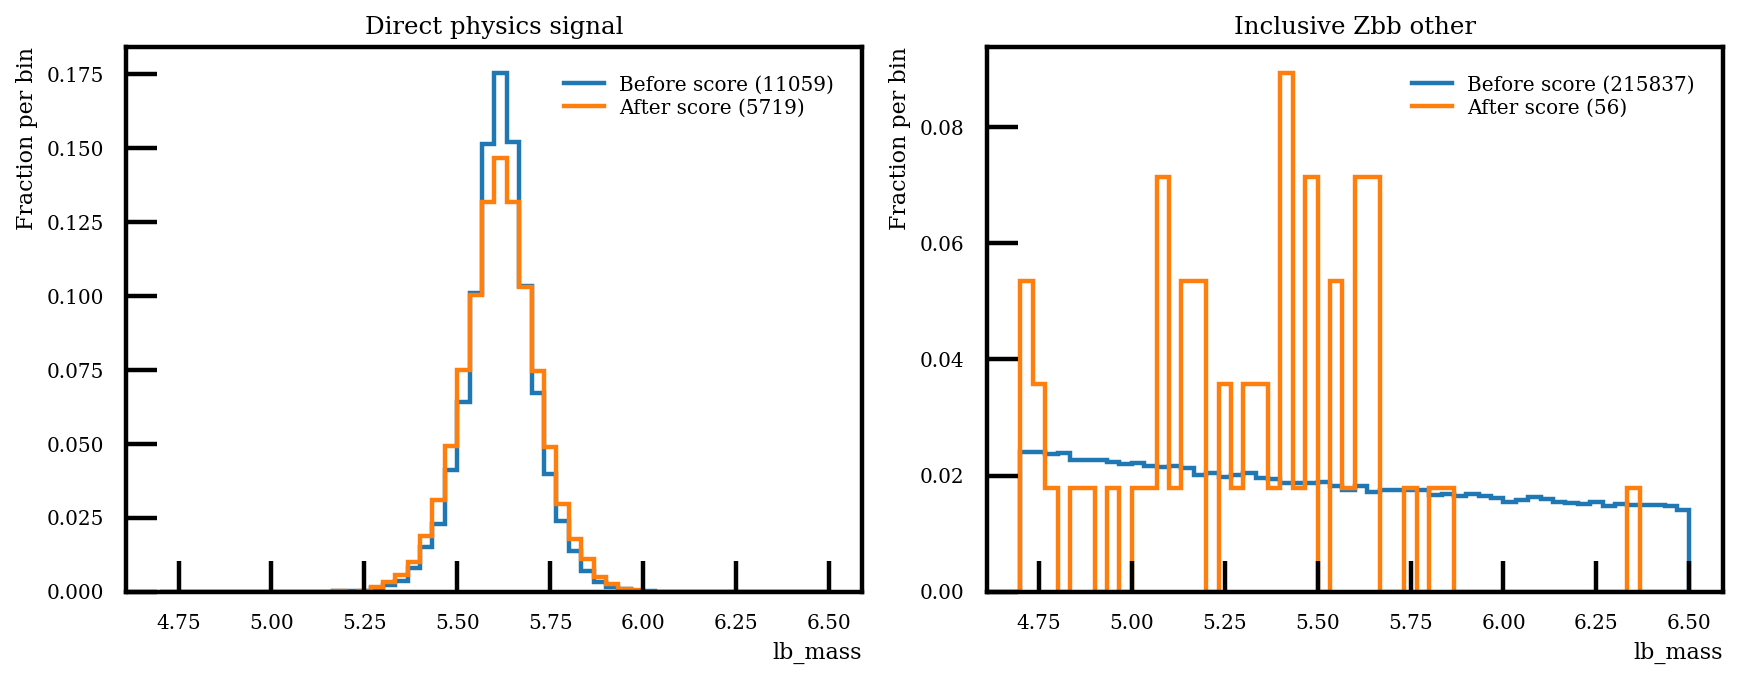
\includegraphics[width=.93\textwidth,height=.43\textheight,keepaspectratio]{mass_before_after_bdt.png}
\smallsource{Mass and angle were excluded from training. Shape checks are required before a mass--angle fit.}
\end{frame}

\begin{frame}{Angular acceptance and next decision}
\begin{columns}[T]
\begin{column}{.58\textwidth}
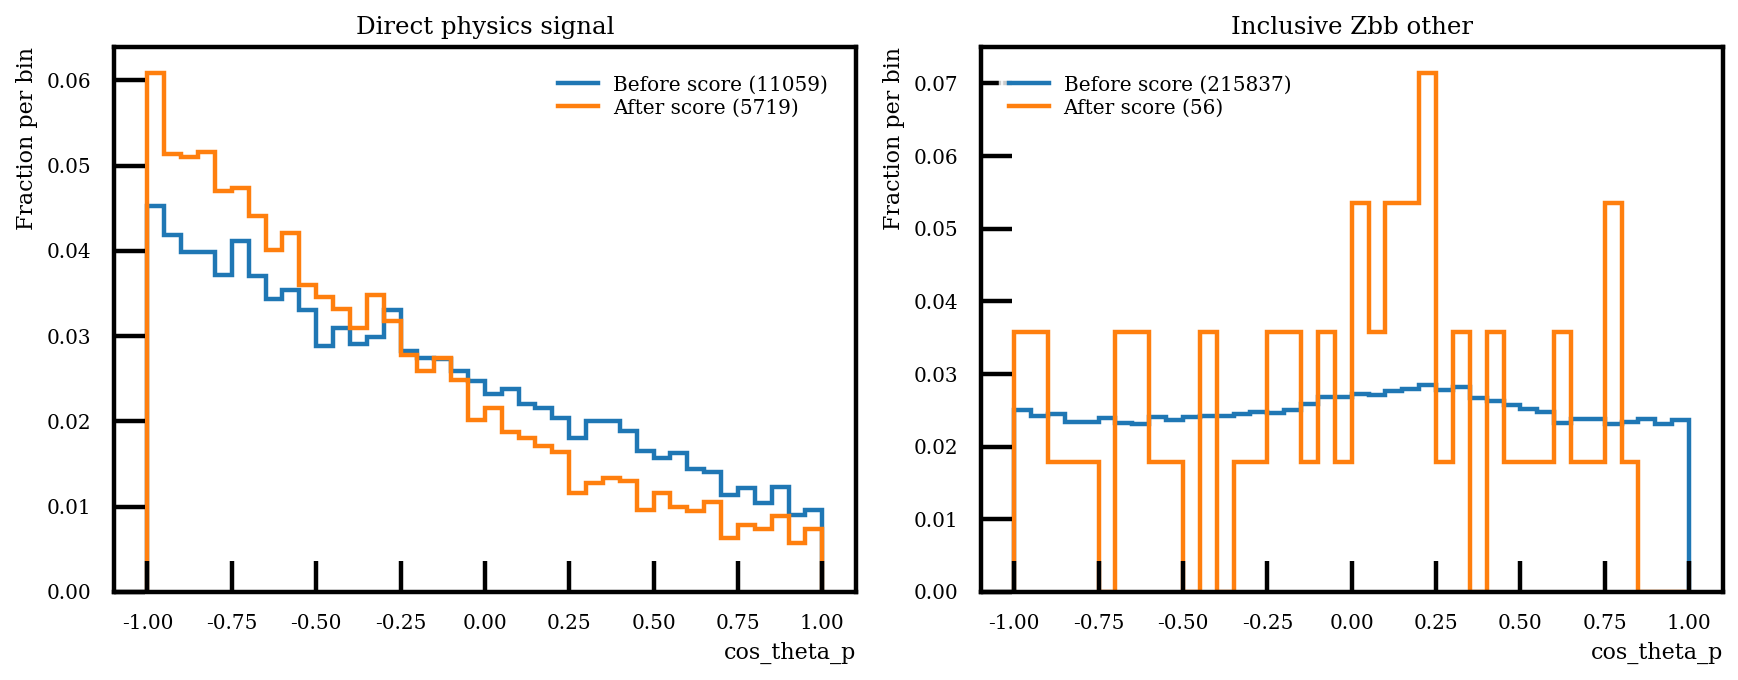
\includegraphics[width=\textwidth]{angle_before_after_bdt.png}
\end{column}
\begin{column}{.4\textwidth}
\small
\begin{itemize}
\item The score changes the direct-signal $\cos\theta_p$ shape through correlated reconstructed inputs.
\item The marked score meets the background ceiling, but central purity is only 26.2\% in the full mass interval.
\item Tighter scores have 11, 6, 3, then 0 validation Zbb survivors in the sampled examples; more background statistics are needed for a high-purity claim.
\item Refresh the remaining Zbb jobs, then process and normalize Zcc/Zss before any mixed-background training.
\end{itemize}
\end{column}
\end{columns}
\smallsource{PI choice pending: specify a purity requirement after reviewing plots. No BDT cut is adopted as the reference selection here.}
\end{frame}
\end{document}
